\chapter{Theory}
\label{ch:theory}

\section{Model: Client/Server}
In the client/server model, as shown in figure \ref{fig:clientservermodel}, every client is only connected to the server. The server transfers data sets to all clients in parallel and thus all clients share the upload bandwidth of the server. This concept does not scale well, because every new client connecting to the system slows down every other client connected to the same server. 

\begin{figure}[H]
\centering
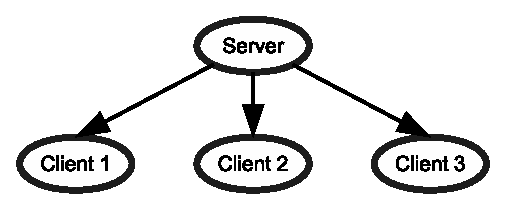
\includegraphics[width=6cm]{clientservermodel}
\caption{Client/Server distribution}
\label{fig:clientservermodel}
\end{figure}

If $b$ is the bandwidth of the server in bytes/second, $n$ the number of clients connected to the server and $s$ the size of the whole data set, then $T= n \cdot T_0$ is the time in seconds it would take to transfer the data set to all clients, where $T_0=\frac{s}{b}$ is the time in seconds for a single tranfser from the server to a client. This formula assumes, that the download bandwidth of each client is bigger than the shared upload bandwidth. This assumption applies to all models presented in this chapter. In reality this makes sense, because clients often have a much higher download bandwidth than upload bandwidth. Without adding servers or using the upload bandwidth of the clients this linear relationship cannot be removed. This traditional model is implemented in the Sequential algorithm, which can be found in section \ref{subsubsec:sequential}.

From the very first beginning it was clear, that this model is not able to keep the limit of $2 \cdot T_0$ seconds but it is implemented to show the immense difference. The next section \ref{subsubsec:logarithmicmodel} presents a much better model.

\pagebreak
\section{Model: Logarithmic}
\label{subsubsec:logarithmicmodel}
If a P2P network is used instead of a client/server model, where every participant is called a peer and has a connection to one or more other peers in the network. The number of connections depends on the used topology. In this thesis only the mesh topology is of importance, as shown in figure \ref{fig:peermesh}, where every peer is connected to every other peer in the network.

\begin{figure}[H]
\centering
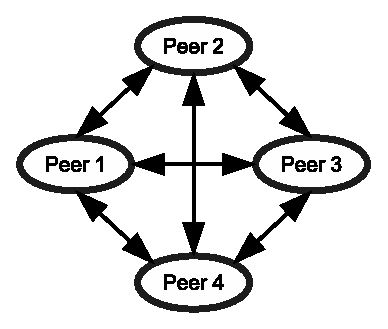
\includegraphics[width=6cm]{peermesh}
\caption{Peer mesh}
\label{fig:peermesh}
\end{figure}

In the logarithmic model every peer can do both uploading and downloading data sets. The only restriction is, that it can only upload to one other peer in parallel. So if a new data set is announced by one peer in the P2P network, all peers try to download this data set from the given peer. Only one peer, basically the first one, is allowed to download the data set. The rest of the requesting peers are rejected and do nothing after this. When the peer completed the download, there are two peers in the network containing the data set. This time another two peers will be allowed to download the data set. This way the number of downloading peers is doubled every $T_0 = \frac{s}{u}$ seconds, where $u$ is the upload bandwidth of each peer, which is considered exponential growth. 

At first, this concept might seem even worse than the client/server model, but it turns out, that this model guarantees, that in $T=\log{(n)} \cdot T_0$  seconds every peer has the complete data set. This formula assumes that every peer has the same upload bandwidth $u$, which is not common in real world situations. But it can illustrate the relationship between the upload bandwidth and the number of peers. The figure \ref{fig:logarithmicmodel} shows 4 peers, where peer 1 is the only peer with the data set at first. It transfers the data set to peer 2 in $T_0$ seconds. Then peer 1 and 2 transfers this data set to peer 3 and 4 respectively in $T_0$ seconds. So the whole transfer takes $2 \cdot T_0$ seconds.

\begin{figure}[H]
\centering
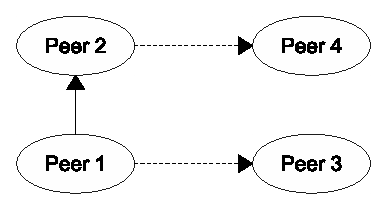
\includegraphics[width=6cm]{logarithmicmodel}
\caption{Logarithmic distribution}
\label{fig:logarithmicmodel}
\end{figure}

The implementation of this model increases the complexity only marginal, but the efficiency is significantly higher. The more peers there are participating the higher is the efficiency. The overhead is also very manageable because during the transfers the idle peers do nothing except waiting. The problem of this model is that never more than 50\% of all peers are uploading in parallel. Also at the beginning only one peer uploads the data set. This means that in the beginning a majority of all peers do not use their upload bandwidth. This model is implemented in the Logarithmic algorithm, which can be found in section \ref{subsubsec:logarithmic}.

At the end this model cannot provide the $2 \cdot T_0$ limit we are looking for. To do so this model has to be improved, which is done in the next section \ref{subsubsec:chunkedswarmmodel}.


\section{Model: Chunked-Swarm}
\label{subsubsec:chunkedswarmmodel}
The Chunked-Swarm model is an enhancement of the logarithmic model. It allows multiple uploads in parallel and splits the data set into chunks before transferring it. So peers cannot download the whole data set at once, but have to request each chunk individually instead. Since the size of those chunks is smaller than the size of the whole data set, the peers can help to distribute the data set more quickly. The figure \ref{fig:chunkedswarmmodel} shows 4 peers distributing 3 chunks. At first peer 1 has the data set completely. Peer 2, 3 and 4 each request one chunk in parallel. Those peers will then distribute their chunks among themselves. This means that those peers announce their own chunks to the other peers, which can then request those chunks. It is important to note, that this model is always pull-based. A chunk is only uploaded if a peer explicitly requests it.

\begin{figure}[H]
\centering
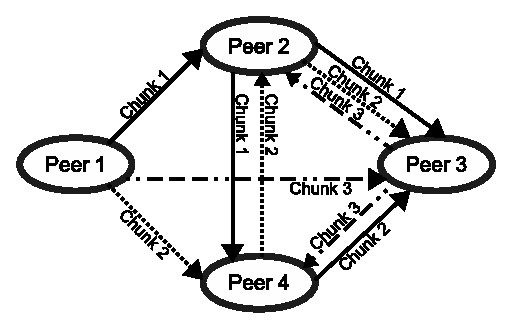
\includegraphics[width=6cm]{chunkedswarmmodel}
\caption{Chunked-Swarm distribution}
\label{fig:chunkedswarmmodel}
\end{figure}

The implementation of this model is not as easy as the logarithmic one, because the efficiency totally depends on the choice of the chunks the peer 2, 3 and 4 request from peer 1. Since this approach is pull-based, the peers do not know what the other peers request. This could lead to chunk duplication which decreases the efficiency considerably. Chunk duplication means that two peers request the same chunk from peer 1 and therefore cannot exchange those chunks afterwards. An implementation of this model has to make strong considerations about this issue. This model is implemented in the ChunkedSwarm and the SuperSeederChunkedSwarm algorithm, which can be found in section \ref{subsubsec:chunkedswarm} and \ref{subsubsec:superseederchunkedswarm} respectively. Those sections also explain the problem of chunk selection in more detail.

To determine the efficiency of this model, it is assumed, that the chunk selection works perfectly, which means that all peers request distinct chunks from peer 1. This also implies that there have to be at least as many chunks as there are peers. Less chunks would also work, but then chunk duplication cannot be prevented.

For simplicity it is also assumed, that there are just as many chunks as there are peers. It this case, it would take $T_0$ seconds to transfer all distinct chunks to all peers, because every peer gets a third of the available bandwidth and also has to download a third of the whole data set. After this, the peers distribute their chunks among themselves, which takes $\frac{2}{3} \cdot T_0$ seconds, as shown in figure \ref{fig:chunkedswarmformula1}.

\begin{figure}[H]
\centering
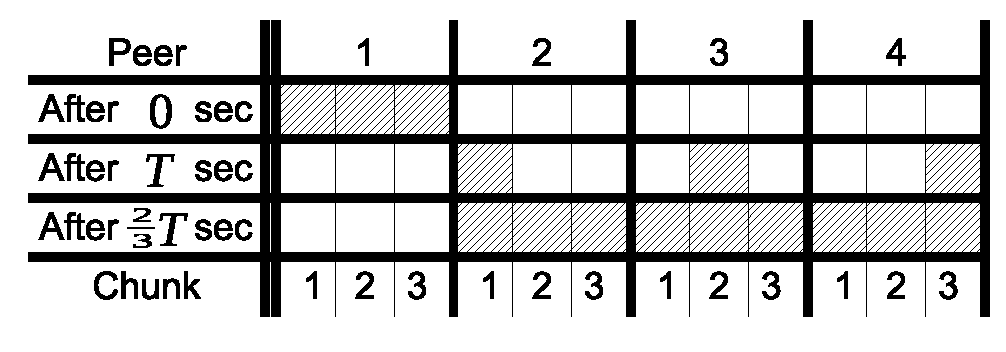
\includegraphics[width=12cm]{chunkedswarmformula1}
\caption{Chunk completion diagramm of the Chunked-Swarm distribution 1}
\label{fig:chunkedswarmformula1}
\end{figure}

This means that after $T = T_0 + \frac{2}{3} \cdot T_0 = \frac{5}{3} \cdot T_0$ seconds every peer has all chunks available. Similiary a variable number of peers need $T(n) = T_0 + \frac{n - 1}{n} \cdot T_0 = \frac{2n - 1}{n} \cdot T_0 = (2 - \frac{1}{n}) \cdot T_0$ seconds. A very nice property of this formula is that the result is always smaller than $2 \cdot T_0$. Without any further optimizations the main objective of this thesis is already fulfilled, as long as the chunk count is equal to or greater than the peer count.

If the chunk count is doubled, the formula gets even better. Figure \ref{fig:chunkedswarmformula2} illustrates this scenario. The efficiency rises because the peers can start to upload their own chunks earlier. After $\frac{1}{2} \cdot T_0$ seconds the peers received the first three distinct chunks from peer 1. At this point the peers can exchange their chunks, which takes $\frac{1}{3} \cdot T_0$ seconds. So after $\frac{5}{6} \cdot T_0$ seconds all peers have the first 50\% of the data set. At $T$ seconds the last three distinct chunks arrive which will also be exchanged afterwards. So after $T = T_0 + \frac{1}{3} \cdot T_0 = \frac{4}{3} \cdot T_0$ seconds all peers have the data set.

\begin{figure}[H]
\centering
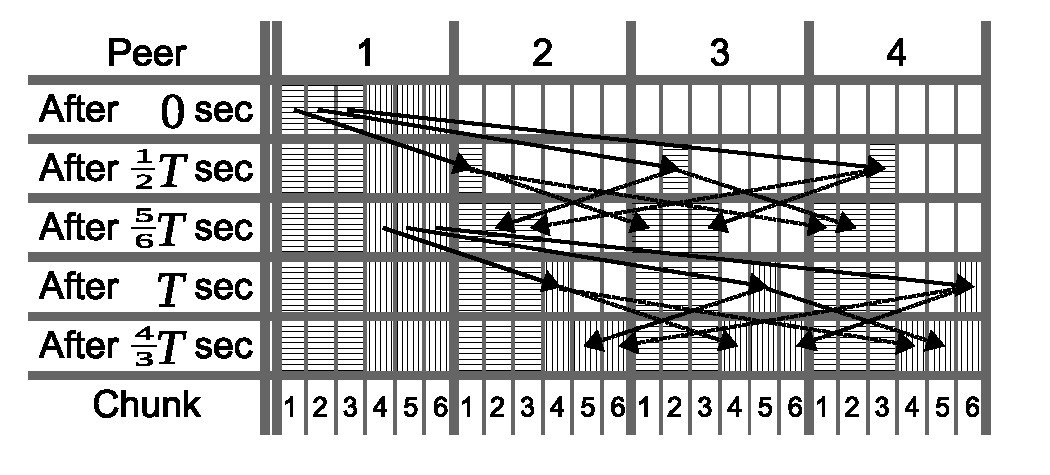
\includegraphics[width=12cm]{chunkedswarmformula2}
\caption{Chunk completion diagramm of the Chunked-Swarm distribution 2}
\label{fig:chunkedswarmformula2}
\end{figure}
